%%%%%%%%%%%%%%%%%%%%%%%%%%%%%%%%%%%%%%%%%%%%%%%%%%%%%%%%%%%%%%%%%%%%%%%
\chapter{PCB Design of a Low-Cost White Noise Generator}

\section{Introduction}

Printed Circuit Boards (PCBs) are widely used in modern electronic systems because they provide a compact, reliable, and permanent platform for electronic circuits. Compared to breadboard implementations, PCBs improve circuit stability, reduce unwanted wiring, and make the circuit easier to manufacture and maintain.

During this internship, a low-cost White Noise Generator PCB was designed using \textbf{KiCad}, an open-source Electronic Design Automation (EDA) software. The objective of this work was to convert an existing white noise generator circuit into a compact and manufacturable PCB design by following standard PCB design practices.

The work included schematic capture, component selection, footprint assignment, PCB layout design, component placement, copper trace routing, design verification, and 3D visualization of the final board. Since the scope of this internship was limited to PCB design, fabrication and hardware testing were not performed.

The final PCB layout serves as a ready-to-manufacture prototype and provides the foundation for future fabrication, assembly, and experimental evaluation.

%%%%%%%%%%%%%%%%%%%%%%%%%%%%%%%%%%%%%%%%%%%%%%%%%%%%%%%%%%%%%%%%%%%%%%%

\section{Objectives}

The main objectives of this work are listed below.

\begin{itemize}

\item Study the working principle of a low-cost white noise generator.

\item Recreate the circuit schematic using KiCad.

\item Select suitable electronic components and PCB footprints.

\item Design a compact and manufacturable PCB layout.

\item Perform proper component placement and copper trace routing.

\item Verify the PCB design using Electrical Rule Check (ERC) and Design Rule Check (DRC).

\item Generate a 3D model of the PCB for visual inspection.

\item Prepare the PCB design for future fabrication.

\end{itemize}

%%%%%%%%%%%%%%%%%%%%%%%%%%%%%%%%%%%%%%%%%%%%%%%%%%%%%%%%%%%%%%%%%%%%%%%

\section{System Overview}

The White Noise Generator is an analog electronic circuit designed to generate a broadband random noise signal. Such signals are commonly used in communication systems, electronic testing, audio applications, and laboratory experiments.

In this project, the complete circuit was designed in KiCad by first creating the schematic and then converting it into a PCB layout. Appropriate component footprints were assigned, the PCB was routed, and the design was verified before generating a 3D model of the board.

%Circuit diagram%

Figure~\ref{fig:white_noise_schematic} presents the reference circuit schematic used for designing the PCB. The original circuit was adapted from Reference~\cite{white_noise_appnote}.

\begin{figure}[H]
\centering
\resizebox{1\textwidth}{!}{%  % Scale the entire circuit to fit text width
\begin{circuitikz}
\tikzstyle{every node}=[font=\fontsize{18.2pt}{23.7pt}\selectfont]  % Set global font size for all nodes

% ===== ZENER DIODE (Voltage Regulator) =====
% Draws the 1N759 zener diode that regulates the +14V supply
\draw (3,6.25) to[empty Zener diode,l={ \fontsize{9.1pt}{11.8pt}\selectfont 1N759}] (3,8.875);

% ===== FIRST OP-AMP (MAX2650 LNA #1) =====
% Position: x=7.625, y=5.75
\draw (7.625,5.75) node[op amp,scale=1, yscale=-1] (opamp2) {};
\draw (opamp2.+) to[short] (6.125,6.25);   % Non-inverting input (+) connection
\draw (opamp2.-) to[short] (6.125,5.25);   % Inverting input (-) connection
\draw (opamp2.out) to[short] (9.125,5.75); % Output connection
\draw (7.625,6.25) -- (7.625,6.75);        % Vcc connection (top)
\draw (7.625,5.25) -- (7.625,4.75);        % GND connection (bottom)

% ===== SECOND OP-AMP (MAX2650 LNA #2) =====
% Position: x=10.625, y=5.875 (cascaded after first LNA)
\draw (10.625,5.875) node[op amp,scale=1, yscale=-1] (opamp2) {};
\draw (opamp2.+) to[short] (9.125,6.375);
\draw (opamp2.-) to[short] (9.125,5.375);
\draw (opamp2.out) to[short] (12.125,5.875);
\draw (10.625,6.375) -- (10.625,6.875);
\draw (10.625,5.375) -- (10.625,4.875);

% ===== RESISTOR (R1 - 30Ω) =====
% Pull-up resistor from +14V to the zener/input node
\draw (3,3.375) to[R,l={ \fontsize{9.1pt}{11.8pt}\selectfont 30 $\Omega$}] (3,6.375);

% ===== INPUT COUPLING CAPACITOR (C1 = 470pF) =====
% AC coupling capacitor between zener node and first LNA input
\draw [line width=0.5pt](6.125,6.25) to[C,l={ \fontsize{9.1pt}{11.8pt}\selectfont 470pF}] (3,6.25);

% ===== INTER-STAGE CONNECTION =====
% Connect first LNA output to second LNA input
\draw (9.125,5.75) to[short] (9.125,6.375);

% ===== INTER-STAGE CAPACITOR (C2 = 470pF) =====
% AC coupling between LNA stages
\draw (14.375,5.875) to[C,l={ \fontsize{9.1pt}{11.8pt}\selectfont 470pF}] (12,5.875);

% ===== DECOUPLING CAPACITOR (C3 = 0.1µF) =====
% Bypass capacitor for +5V supply noise filtering
\draw (14.875,8)
to[C,l={\fontsize{9.1pt}{11.8pt}\selectfont $0.1\,\mu\mathrm{F}$}]
(12.75,8);

% ===== POWER SUPPLY DISTRIBUTION =====
% +5V power rail for both LNAs
\draw (5.625,8) to[short] (12.75,8);
\draw (7.625,6.75) to[short] (7.625,8);    % Vcc to first LNA
\draw (10.625,6.875) to[short] (10.625,8); % Vcc to second LNA

% ===== GROUNDING =====
% Ground connection for C3
\draw (14.875,8) to (14.875,7.875) node[ground]{};

% ===== THIRD OP-AMP (Duplicate - Appears to be redundant) =====
% WARNING: This seems to be a duplicate drawing error

% ===== REPEATED OP-AMP (MORE DUPLICATES) =====
% These appear to be copy-paste errors - should be removed


% ===== REPEATED OP-AMP AGAIN =====
% SAME DUPLICATE - Remove this entire block


% ===== ARROWS INDICATING SUPPLY VOLTAGES =====
% Arrows pointing to voltage labels
\draw [-{Stealth[scale=1.5]}, ] (5.625,8) -- (5.625,9);  % +5V arrow
\draw [-{Stealth[scale=1.5]}, ] (3,8.375) -- (3,9);      % +14V arrow

% ===== GROUND FOR R1 =====
\draw (3,4.25) to (3,3.375) node[ground]{};

% % ===== MORE REPEATED OP-AMP (DUPLICATE) =====
% % Yet another duplicate - remove this

% ===== OUTPUT MARKER =====
% White circle marking output node (indicates output connection)
\draw [ fill={rgb,255:red,255; green,255; blue,255}, fill opacity=1] (14.5,5.875) circle (0.25cm);

% ===== VOLTAGE LABELS =====
% Power supply labels
\node [font=\fontsize{9.1pt}{11.8pt}\selectfont, inner xsep=0.080cm, inner ysep=0.085cm, rounded corners=0.020cm] at (2.875,9.25) {+14V};
\node [font=\fontsize{9.1pt}{11.8pt}\selectfont, inner xsep=0.080cm, inner ysep=0.085cm, rounded corners=0.020cm] at (5.625,9.25) {+5V};

% ===== I/O LABELS =====
\node [font=\fontsize{9.1pt}{11.8pt}\selectfont, inner xsep=0.080cm, inner ysep=0.085cm, rounded corners=0.020cm] at (6.25,6.5) {IN};      % Input label
\node [font=\fontsize{9.1pt}{11.8pt}\selectfont, inner xsep=0.080cm, inner ysep=0.085cm, rounded corners=0.020cm] at (5.25,4.5) {GND};    % Ground label
\node [font=\fontsize{9.1pt}{11.8pt}\selectfont, inner xsep=0.080cm, inner ysep=0.085cm, rounded corners=0.020cm] at (7.875,7.5) {Vcc};   % Vcc pin label for LNA1
\node [font=\fontsize{9.1pt}{11.8pt}\selectfont, inner xsep=0.080cm, inner ysep=0.085cm, rounded corners=0.020cm] at (8.5,5.5) {OUT};    % Output label for LNA1
\node [font=\fontsize{9.1pt}{11.8pt}\selectfont, inner xsep=0.080cm, inner ysep=0.085cm, rounded corners=0.020cm] at (10.875,7.375) {Vcc}; % Vcc pin label for LNA2
\node [font=\fontsize{9.1pt}{11.8pt}\selectfont, inner xsep=0.080cm, inner ysep=0.085cm, rounded corners=0.020cm] at (11.625,5.625) {OUT}; % Output label for LNA2

% ===== COMPONENT REFERENCE LABELS =====
\node [font=\fontsize{9.1pt}{11.8pt}\selectfont, inner xsep=0.080cm, inner ysep=0.085cm, rounded corners=0.020cm] at (2.125,5.5) {R1};    % Resistor label
\node [font=\fontsize{9.1pt}{11.8pt}\selectfont, inner xsep=0.080cm, inner ysep=0.085cm, rounded corners=0.020cm] at (4.5,6.875) {C1};   % Capacitor label
\node [font=\fontsize{9.1pt}{11.8pt}\selectfont, inner xsep=0.080cm, inner ysep=0.085cm, rounded corners=0.020cm] at (13.75,8.5) {C3};   % Decoupling cap label
\node [font=\fontsize{9.1pt}{11.8pt}\selectfont, inner xsep=0.080cm, inner ysep=0.085cm, rounded corners=0.020cm] at (13.125,6.375) {C2}; % Inter-stage cap label
\node [font=\fontsize{9.1pt}{11.8pt}\selectfont, inner xsep=0.080cm, inner ysep=0.085cm, rounded corners=0.020cm] at (9.375,6.625) {IN};  % Input label for LNA2

% ===== GROUND RAIL (Common ground connection) =====
\draw [short] (6.125,4.25) -- (10.625,4.25);  % Ground bus for both LNAs
\draw [short] (6.125,5.25) -- (6.125,4.25);   % LNA1 inverting input to ground
\draw [short] (7.625,4.875) -- (7.625,4.25);  % LNA1 output ground
\draw [short] (9.125,5.375) -- (9.125,4.25);  % LNA2 inverting input to ground
\draw [short] (10.625,5) -- (10.625,4.25);    % LNA2 output ground
\draw (6.125,4.25) to (5.125,4.25) node[ground]{}; % Final ground connection

% ===== REPEATED OP-AMP (ANOTHER DUPLICATE) =====
% REMOVE THIS DUPLICATE

% ===== IC LABELS =====
\node [font=\fontsize{9.1pt}{11.8pt}\selectfont, inner xsep=0.080cm, inner ysep=0.085cm, rounded corners=0.020cm] at (7,3.75) {MAX2650 (1)};   % LNA1 label
\node [font=\fontsize{9.1pt}{11.8pt}\selectfont, inner xsep=0.080cm, inner ysep=0.085cm, rounded corners=0.020cm] at (10,3.75) {MAX2650 (2)}; % LNA2 label

% ===== BORDER (Figure frame) =====
% Rectangular border around the entire circuit
\draw  (1.375,10.25) rectangle (15.875,2.25);

\end{circuitikz}
}
%  % End of resizebox

\caption{Circuit schematic of the White Noise Generator using two MAX2650 low-noise amplifiers.}
\label{fig:white_noise_schematic}
\end{figure}
%%%%%%%%%%%%%%%%%%%%%%%%%%%%%%%%%%%%%%%%%%%%%%%%%%%%%%%%%%%%%%%%%%%%%%%

\section{Working Principle of the White Noise Generator}

White noise is a random electrical signal that contains a wide range of frequency components with nearly uniform power over a specified frequency range. Due to its broadband nature, white noise is commonly used in communication systems, electronic testing, filter characterization, and audio applications.

The white noise generator designed in this project is based on the avalanche breakdown phenomenon of a reverse-biased Zener diode. When the reverse voltage applied across the Zener diode exceeds its breakdown voltage, random movement of charge carriers produces a very small electrical noise signal. Although this signal has the characteristics of white noise, its amplitude is too low for practical use.

To obtain a usable output, the generated noise signal is amplified using three cascaded MAX2650 low-noise amplifier (LNA) stages. These amplifiers increase the signal amplitude while maintaining a wide operating bandwidth. A regulated +5\,V power supply, provided by the LM2940 voltage regulator, ensures stable operation of the active components. In addition, an adjustable reference circuit using the AZ9431BQ shunt regulator and TS53 trimmer allows the operating point of the Zener diode to be fine-tuned.

\begin{figure}[H]
    \centering
    \setlength{\fboxsep}{0pt}      % No padding
    \setlength{\fboxrule}{0.6pt}   % Border thickness
    %\fbox{%
        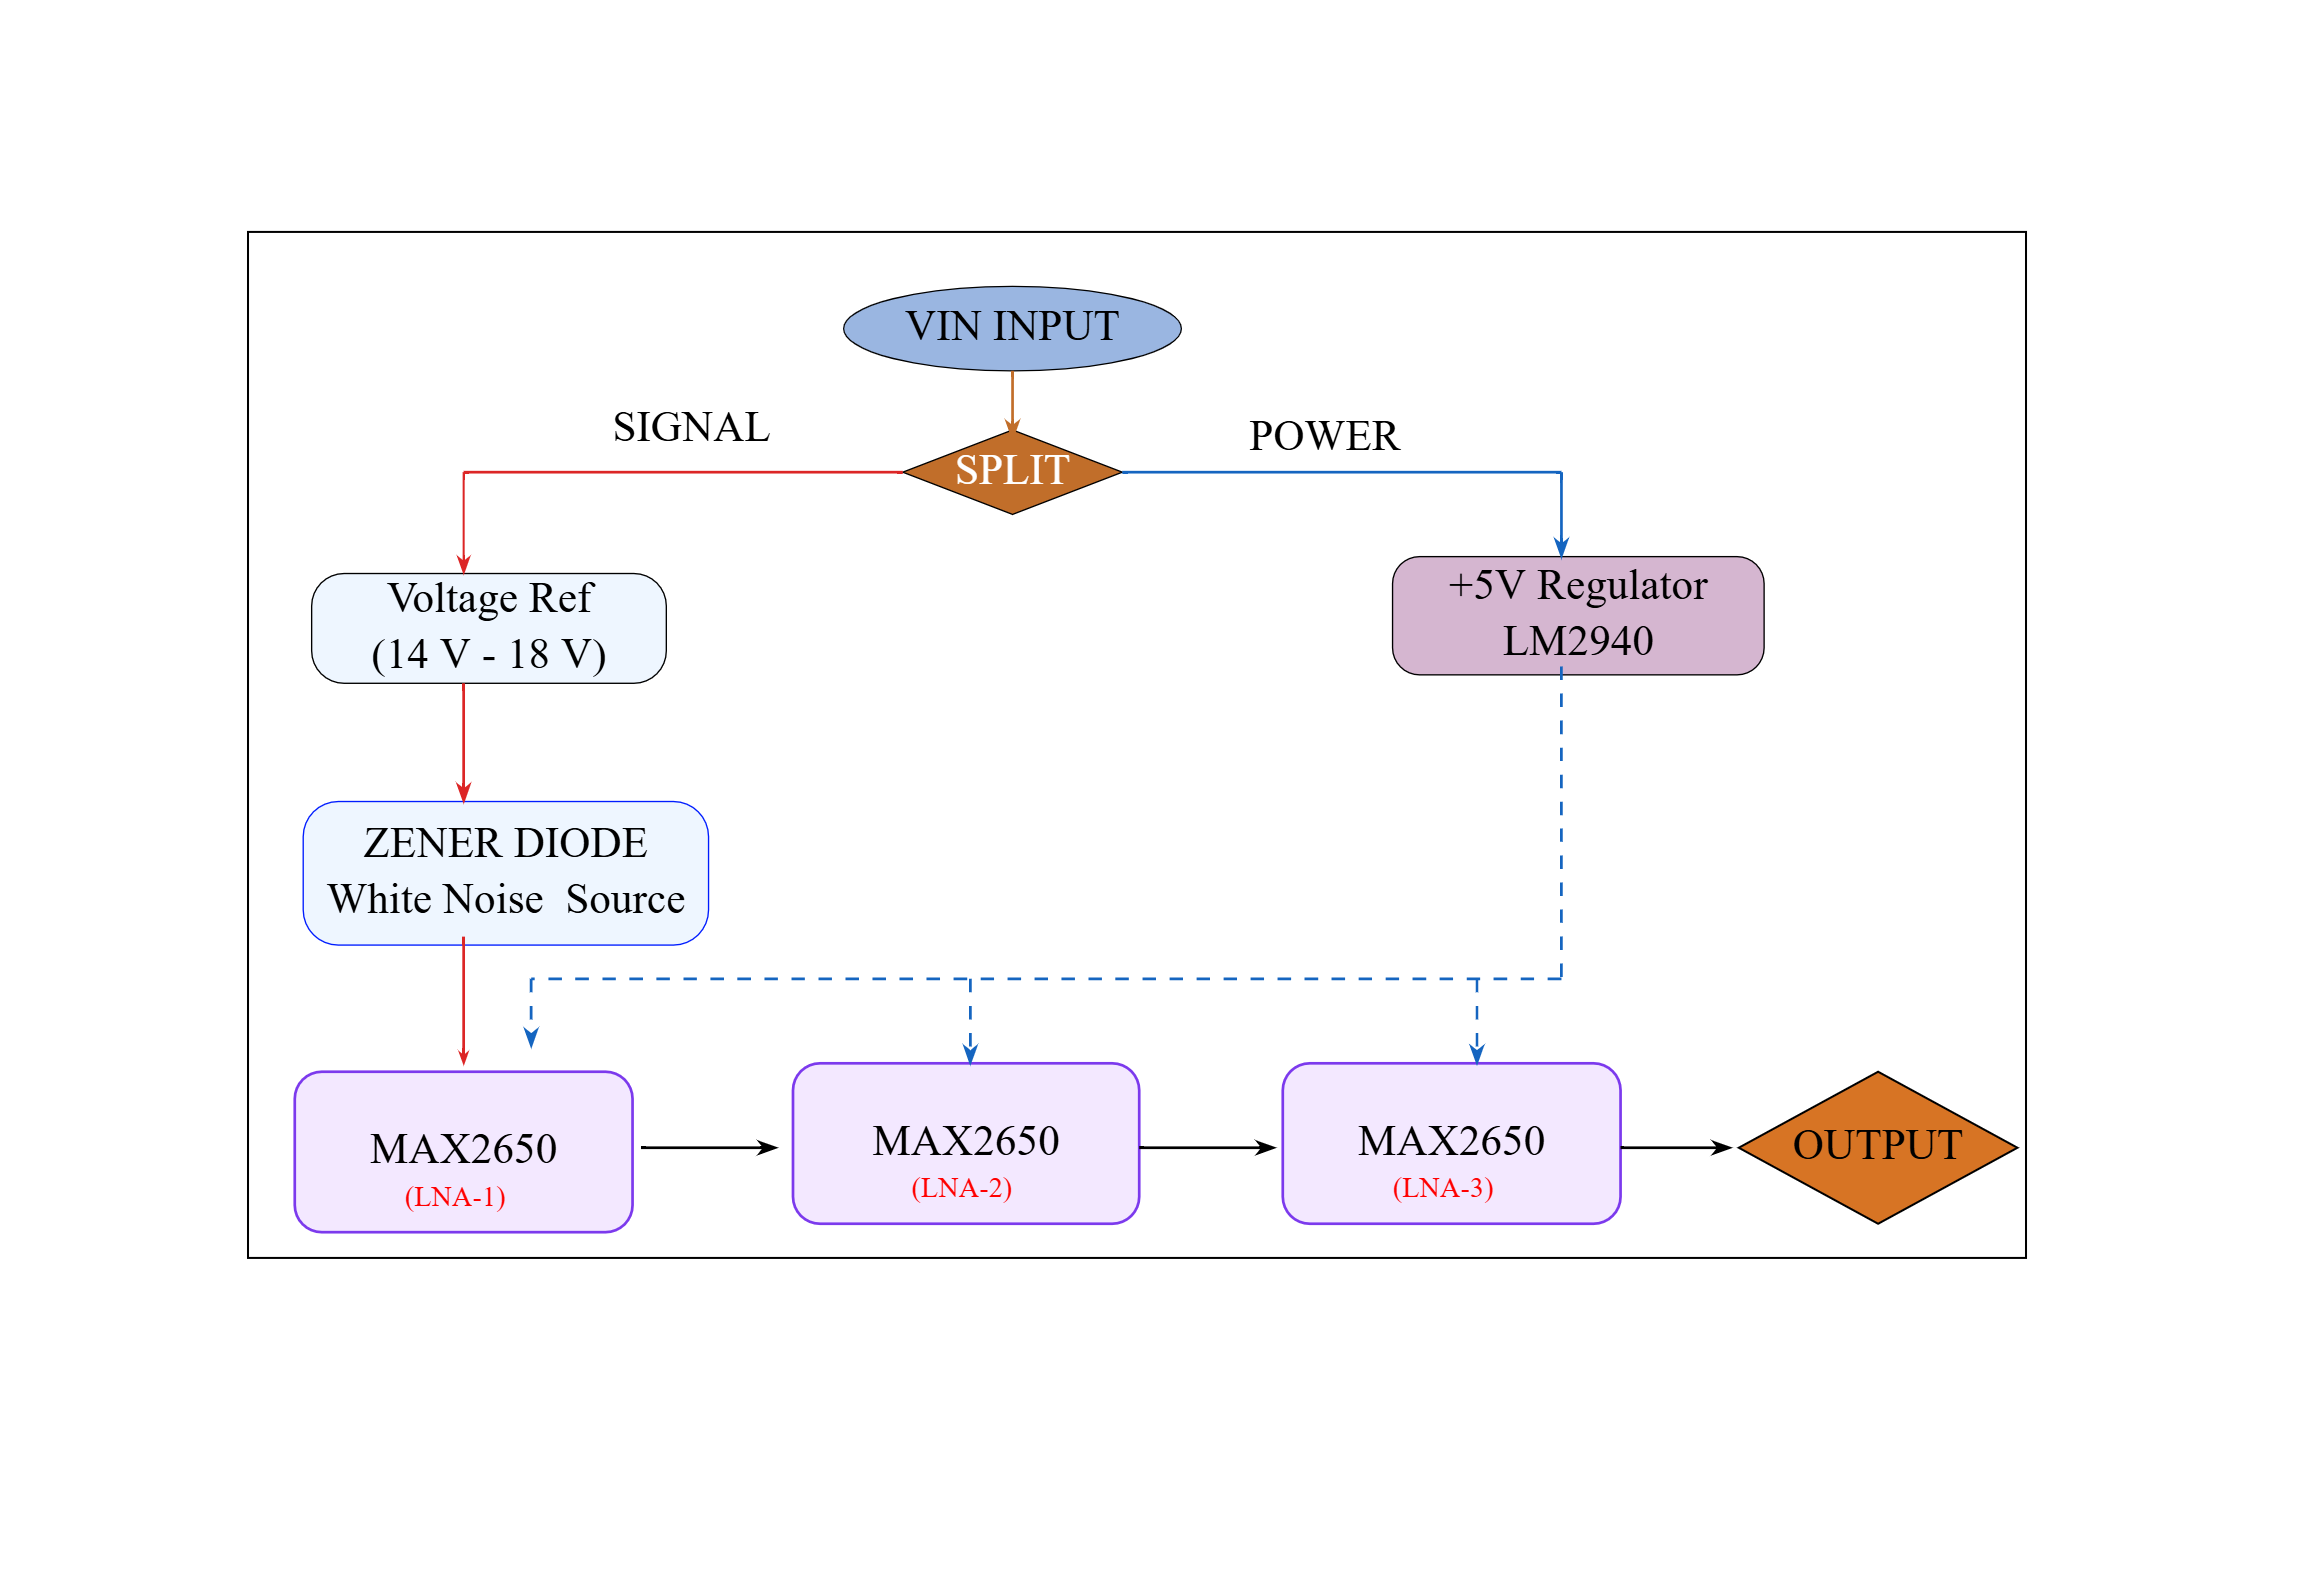
\includegraphics[
            width=0.8\textwidth,
            trim=10cm 11.5cm 10.5cm 10.0cm,
            clip
        ]{projects_records/White_Noice_Gen/Version3.0/circuit (3).png}
    %}
    \caption{Functional Block Diagram of the White Noise Generator}
    \label{fig:white_noise}
\end{figure}



%%%%%%%%%%%%%%%%%%%%%%%%%%%%%%%%%%%%%%%%%%%%%%%%%%%%%%%%%%%%%%%%%%%%%%%


\section{Circuit Schematic Design}

The circuit schematic was developed using the KiCad Electronic Design Automation (EDA) software. The objective of the schematic design was to accurately represent all electrical connections of the white noise generator before proceeding to PCB layout design.

The schematic consists of four main functional blocks: the power supply, bias and reference circuit, white noise generation stage, and amplifier stage. Each block performs a specific function and together they generate and amplify the white noise signal.

The design process began by placing the required electronic components in the KiCad schematic editor. Appropriate symbols were selected from the KiCad component libraries, and all electrical connections were completed according to the circuit design. Power symbols, ground connections, and net labels were added to improve readability and simplify circuit verification.

After completing the schematic, an Electrical Rule Check (ERC) was performed to identify missing connections, incorrect pin configurations, or other electrical errors. All reported issues were corrected before proceeding to the PCB layout stage.

The completed schematic of the White Noise Generator is shown in Figure~\ref{fig:white_noise_schematic2}.

\begin{figure}[H]
    \centering
    \begin{adjustbox}{frame, trim={10 140 10 140}, clip}
        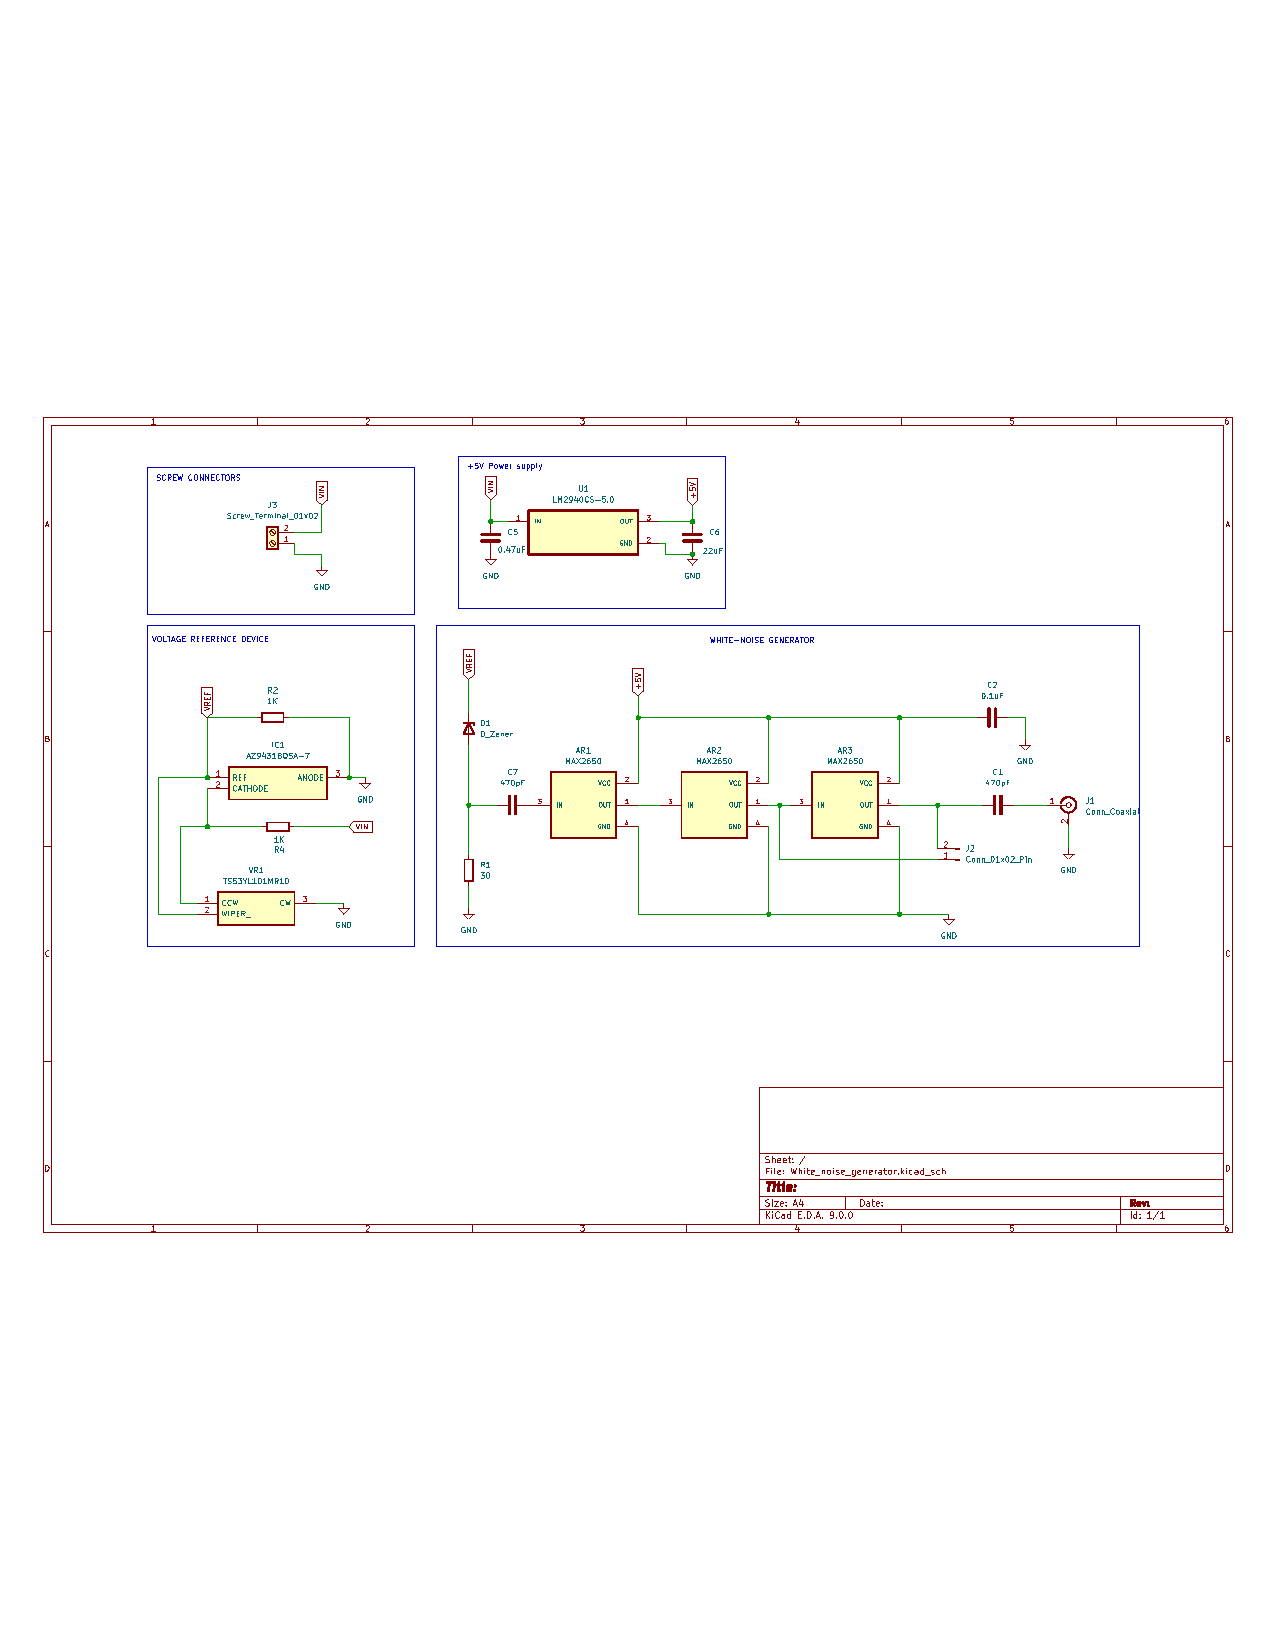
\includegraphics[width=\textwidth]{projects_records/White_Noice_Gen/Version3.0/Schematic_pdf.pdf}
    \end{adjustbox}
    \caption{Noise Generator Circuit - Schematic}
    \label{fig:white_noise_schematic2}
\end{figure}

%%%%%%%%%%%%%%%%%%%%%%%%%%%%%%%%%%%%%%%%%%%%%%%%%%%%%%%%%%%%%%%%%%%%%%%

\subsection{Functional Blocks of the Circuit}

The complete circuit can be divided into four functional blocks, each responsible for a specific operation.

\begin{enumerate}

\item \textbf{Power Supply Block}

The LM2940 voltage regulator converts the input supply into a stable +5\,V output required by the active components of the circuit.

\item \textbf{Bias and Reference Circuit}

The AZ9431BQ precision shunt regulator and TS53 trimmer establish the operating voltage for the reverse-biased Zener diode, ensuring stable noise generation.

\item \textbf{White Noise Generation Block}

The reverse-biased Zener diode operates in avalanche breakdown mode and generates a low-level broadband white noise signal.

\item \textbf{Amplifier Block}

Three MAX2650 low-noise amplifier stages are connected in cascade to amplify the weak noise signal and produce a usable output.

\end{enumerate}

%%%%%%%%%%%%%%%%%%%%%%%%%%%%%%%%%%%%%%%%%%%%%%%%%%%%%%%%%%%%%%%%%%%%%%%

\section{PCB Design Methodology}

After completing and verifying the circuit schematic, the next step was to design the Printed Circuit Board (PCB) using KiCad. The objective was to develop a compact, well-organized, and manufacturable PCB while following standard PCB design practices.

PCB development involved assigning footprints to all components, arranging them on the board, routing electrical connections, and verifying the completed layout before generating manufacturing files.

%%%%%%%%%%%%%%%%%%%%%%%%%%%%%%%%%%%%%%%%%%%%%%%%%%%%%%%%%%%%%%%%%%%%%%%

\subsection{Footprint Assignment}

Each component in the schematic was assigned an appropriate PCB footprint using the KiCad footprint libraries. The selected footprints matched the package dimensions specified in the respective component datasheets to ensure correct placement during PCB fabrication and assembly.

After assigning footprints, the footprint associations were verified to confirm that every schematic symbol was linked to its corresponding PCB package.

%%%%%%%%%%%%%%%%%%%%%%%%%%%%%%%%%%%%%%%%%%%%%%%%%%%%%%%%%%%%%%%%%%%%%%%

\subsection{PCB Layout Design}

The PCB layout was created by importing the completed schematic into the KiCad PCB Editor. Initially, all components appeared outside the board outline. A suitable board size was selected, and the components were arranged systematically to obtain a compact and organized layout.

The placement was planned to reduce unnecessary routing complexity while maintaining sufficient spacing between components for reliable manufacturing.

Figure~\ref{fig:pcb_layout} shows the completed PCB layout designed in KiCad.

\begin{figure}[H]
    \centering
    \begin{adjustbox}{frame, trim={0 40 1 40}, clip}
        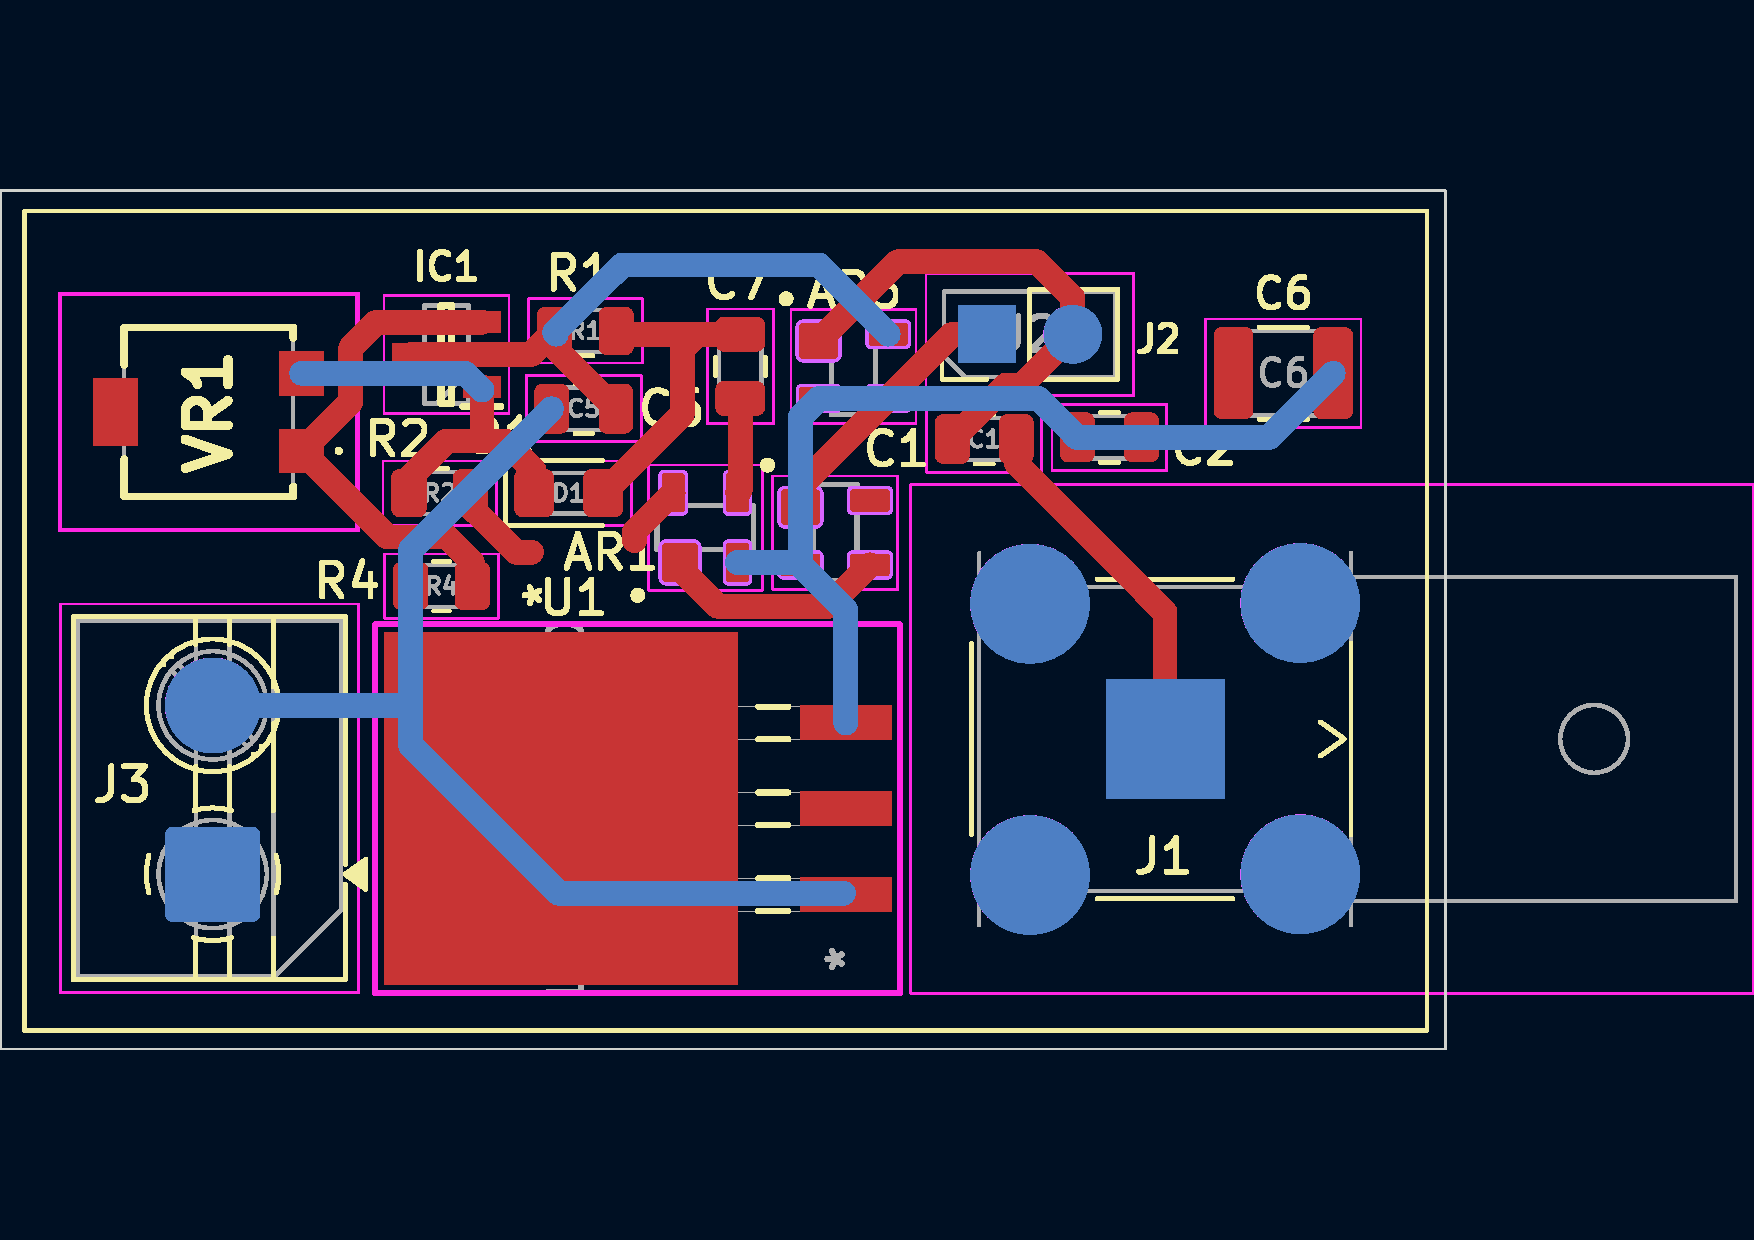
\includegraphics[width=0.84\textwidth]{projects_records/White_Noice_Gen/Version3.0/PCB_layout.pdf}
    \end{adjustbox}
    \caption{Noise Generator- PCB Layout}
    \label{fig:pcb_layout}
\end{figure}

%%%%%%%%%%%%%%%%%%%%%%%%%%%%%%%%%%%%%%%%%%%%%%%%%%%%%%%%%%%%%%%%%%%%%%%

\subsection{Component Placement}

Proper component placement is an important step in PCB design because it directly affects routing quality, board size, and overall circuit performance.

Components performing similar functions were grouped together to simplify routing. The amplifier stages were placed sequentially to maintain the signal flow, while the power supply and biasing components were positioned close to the circuits they support. This arrangement reduced routing complexity and improved the overall organization of the PCB.

%%%%%%%%%%%%%%%%%%%%%%%%%%%%%%%%%%%%%%%%%%%%%%%%%%%%%%%%%%%%%%%%%%%%%%%

\subsection{Copper Trace Routing}

After component placement, electrical connections were completed by routing copper traces between the components. Appropriate trace widths were selected according to the power and signal requirements of the circuit.

Short and direct routing paths were preferred wherever possible to minimize unnecessary trace length. The routing was completed while avoiding overlapping traces and maintaining adequate spacing between adjacent tracks.

%%%%%%%%%%%%%%%%%%%%%%%%%%%%%%%%%%%%%%%%%%%%%%%%%%%%%%%%%%%%%%%%%%%%%%%

\subsection{Ground Plane}

A ground copper pour was added to the PCB to provide a common reference potential for the circuit. The ground plane also improves electrical connectivity and simplifies PCB routing by reducing the number of individual ground traces.

%%%%%%%%%%%%%%%%%%%%%%%%%%%%%%%%%%%%%%%%%%%%%%%%%%%%%%%%%%%%%%%%%%%%%%%

\subsection{Design Verification}

The completed PCB layout was verified using the Design Rule Check (DRC) tool available in KiCad. The verification process checked for routing errors, clearance violations, overlapping tracks, and other manufacturing issues.

After correcting all identified issues, the PCB layout was considered ready for manufacturing file generation.

%%%%%%%%%%%%%%%%%%%%%%%%%%%%%%%%%%%%%%%%%%%%%%%%%%%%%%%%%%%%%%%%%%%%%%%

\subsection{3D PCB Visualization}

KiCad provides a built-in 3D Viewer that allows the designed PCB to be inspected before fabrication. The 3D model was used to verify component placement, footprint orientation, and the overall appearance of the board.

\begin{figure}[H]
\centering

\begin{minipage}{0.48\textwidth}
\centering
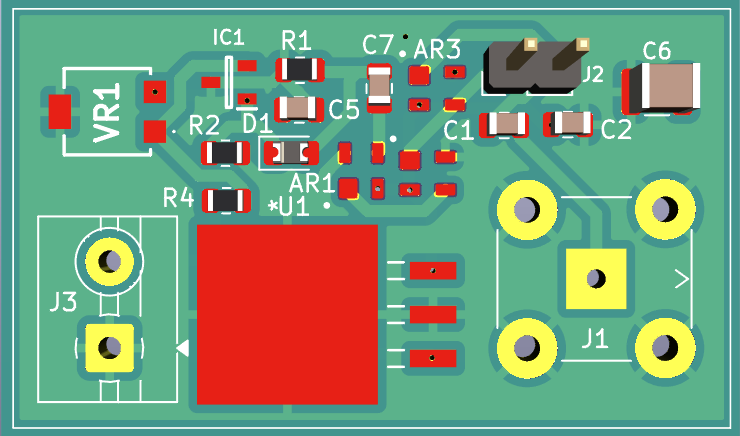
\includegraphics[width=\linewidth]{projects_records/White_Noice_Gen/Version3.0/top_view.png}
\label{fig:top view}
\caption{Top View}
\end{minipage}
\hfill
\begin{minipage}{0.48\textwidth}
\centering
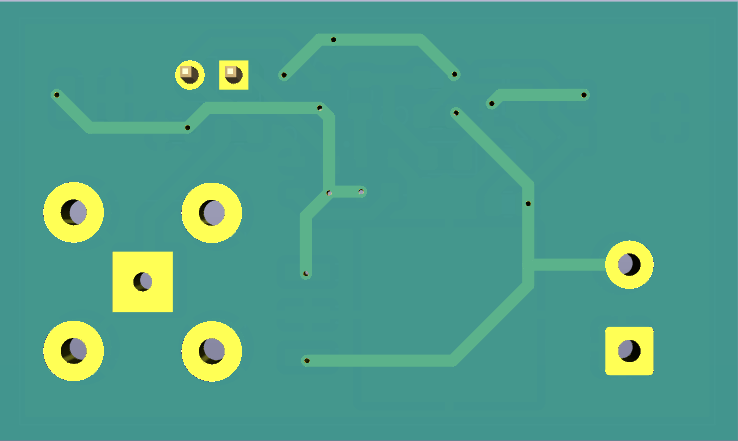
\includegraphics[width=\linewidth]{projects_records/White_Noice_Gen/Version3.0/bottom_view.png}
\label{fig:top and bottom view}

\caption{Bottom View}
\end{minipage}

% \caption{Hardware Setup Used During Experimental Evaluation}
\label{fig:top and bottom view}

\end{figure}

%%%%%%%%%%%%%%%%%%%%%%%%%%%%%%%%%%%%%%%%%%%%%%%%%%%%%%%%%%%%%%%%%%%%%%%
%%%%%%%%%%%%%%%%%%%%%%%%%%%%%%%%%%%%%%%%%%%%%%%%%%%%%%%%%%%%%%%%%%%%%%%

\section{Manufacturing Outputs}

After completing the PCB layout and verifying the design using the Design Rule Check (DRC), the manufacturing files required for PCB fabrication were generated in KiCad. These files prepare the design for future fabrication and assembly. As the primary objective of this internship was PCB design, fabrication and hardware testing were outside the scope of this work.

%%%%%%%%%%%%%%%%%%%%%%%%%%%%%%%%%%%%%%%%%%%%%%%%%%%%%%%%%%%%%%%%%%%%%%%

\subsection{Gerber and Drill Files}

The complete set of Gerber files and NC drill files was generated using KiCad. The Gerber files contain the information for the copper layers, solder mask, silkscreen, and board outline, while the drill files specify the locations and diameters of all drilled holes required during PCB manufacturing.

The generated manufacturing files are included in the project repository and can be directly used for PCB fabrication.

%%%%%%%%%%%%%%%%%%%%%%%%%%%%%%%%%%%%%%%%%%%%%%%%%%%%%%%%%%%%%%%%%%%%%%%

%%%%%%%%%%%%%%%%%%%%%%%%%%%%%%%%%%%%%%%%%%%%%%%%%%%%%%%%%%%%%%%%%%%%%%%

\subsection{Bill of Materials (BOM)}

A Bill of Materials (BOM) was automatically generated using KiCad after completing the PCB design. The BOM lists all components required for PCB assembly, including their reference designators, quantities, component values, and PCB footprints. The complete BOM, along with the Gerber and NC drill files, is available in the project repository.

\begin{table}[H]
\centering
\caption{Bill of Materials (BOM) Generated Using KiCad}
\label{tab:bom}
\renewcommand{\arraystretch}{1.25}
\begin{tabular}{|c|c|l|l|}
\hline
\textbf{Reference} & \textbf{Qty} & \textbf{Value} & \textbf{Footprint} \\
\hline
AR1--AR3 & 3 & MAX2650 & SOT190P228X119-4N \\
\hline
C1, C7 & 2 & 470 pF & 0805 \\
\hline
C2 & 1 & 0.1 $\mu$F & 0805 \\
\hline
C5 & 1 & 0.47 $\mu$F & 0805 \\
\hline
C6 & 1 & 22 $\mu$F & 1210 \\
\hline
D1 & 1 & 1N759 Zener Diode & D\_0805 \\
\hline
IC1 & 1 & AZ9431BQSA-7 & SOT96P240X110-3N \\
\hline
J1 & 1 & BNC Connector & BNC\_WNG1 \\
\hline
J2 & 1 & 2-Pin Header & Pin Header 2.54 mm \\
\hline
J3 & 1 & Screw Terminal & 5.08 mm Terminal Block \\
\hline
R1 & 1 & 30 $\Omega$ & 0805 \\
\hline
R2, R4 & 2 & 1 k$\Omega$ & 0805 \\
\hline
U1 & 1 & LM2940IMP-9.0 & TO254P1524X483-4N \\
\hline
VR1 & 1 & TS53YL101MR10 & TS53 \\
\hline
\end{tabular}
\end{table}

%%%%%%%%%%%%%%%%%%%%%%%%%%%%%%%%%%%%%%%%%%%%%%%%%%%%%%%%%%%%%%%%%%%%%%%
%%%%%%%%%%%%%%%%%%%%%%%%%%%%%%%%%%%%%%%%%%%%%%%%%%%%%%%%%%%%%%%%%%%%%%%
%%%%%%%%%%%%%%%%%%%%%%%%%%%%%%%%%%%%%%%%%%%%%%%%%%%%%%%%%%%%%%%%%%%%%%%

\section{Results and Discussion}

The White Noise Generator PCB was successfully designed using KiCad by following the standard PCB design workflow. The schematic was recreated from the reference circuit, footprints were assigned to all components, and a compact PCB layout was developed.

The completed PCB was verified using Electrical Rule Check (ERC) and Design Rule Check (DRC) to identify and eliminate design errors. A ground plane was added, copper traces were routed, and the final layout was inspected using KiCad's 3D Viewer. Manufacturing outputs, including Gerber files, drill files, and the Bill of Materials (BOM), were generated successfully.

Although the PCB was not fabricated or experimentally tested during the internship, the completed design is suitable for future manufacturing and hardware implementation.

%%%%%%%%%%%%%%%%%%%%%%%%%%%%%%%%%%%%%%%%%%%%%%%%%%%%%%%%%%%%%%%%%%%%%%%

\section{Future Scope}

The work completed during this internship provides a foundation for future development of the White Noise Generator. The following activities can be carried out in future work:

\begin{itemize}
    \item Fabrication of the designed PCB using the generated Gerber files.
    \item Assembly and soldering of all electronic components on the PCB.
    \item Experimental testing and performance evaluation of the circuit.
    \item Measurement of output characteristics using laboratory instruments such as an oscilloscope and spectrum analyzer.
    \item Optimization of the PCB layout to further reduce electrical noise and improve signal quality.
    \item Integration of the White Noise Generator into RF communication and electronic testing applications.
\end{itemize}

%%%%%%%%%%%%%%%%%%%%%%%%%%%%%%%%%%%%%%%%%%%%%%%%%%%%%%%%%%%%%%%%%%%%%%%

\section{Conclusion}

During this internship, the complete PCB design of a White Noise Generator was developed using KiCad. The work included schematic capture, footprint assignment, PCB layout design, component placement, copper trace routing, design verification, 3D visualization, and generation of manufacturing files.

The internship provided practical experience in professional PCB design techniques and the use of modern Electronic Design Automation (EDA) tools. The completed design serves as a manufacturing-ready PCB that can be fabricated and tested in future work.

%%%%%%%%%%%%%%%%%%%%%%%%%%%%%%%%%%%%%%%%%%%%%%%%%%%%%%%%%%%%%%%%%%%%%%%